\documentclass[12pt,a4paper]{article}

\usepackage[a4paper,width=160mm,top=25mm,bottom=25mm]{geometry}

\usepackage{fancyhdr}
\pagestyle{fancy}
\fancyhf{}
\fancyhead[EL]{\nouppercase\leftmark}
\fancyhead[OR]{\nouppercase\rightmark}
\fancyhead[ER,OL]{\thepage}

\usepackage{url}
\usepackage[hidelinks]{hyperref}

\renewcommand{\linethickness}{0.05em}
\usepackage[brazil]{babel}   
\usepackage{titlesec}
\newcommand{\sectionbreak}{\clearpage}


\title{Processando a Informação: um livro prático de programação independente de linguagem 
\\\large\vspace{2cm}
Rogério Perino de Oliveira Neves 
\\\vspace{5mm}
Francisco de Assis Zampirolli
\\\large\vspace{2cm}
EDUFABC
\\ \url{editora.ufabc.edu.br}
\\\Huge\vspace{3cm}
Notas de Aulas inspiradas no livro
\\\Large\vspace{1cm}
Utilizando a(s) Linguagem(ns) de Programação: 
\\\Huge\vspace{1cm}
C
\\\large\vspace{1cm}
Exemplos adaptados para Correção Automática no Moodle+VPL
\vspace{2cm}}
\author{Francisco de Assis Zampirolli\vspace{1cm}}


    \usepackage[breakable]{tcolorbox}
    \usepackage{parskip} % Stop auto-indenting (to mimic markdown behaviour)
    

    % Basic figure setup, for now with no caption control since it's done
    % automatically by Pandoc (which extracts ![](path) syntax from Markdown).
    \usepackage{graphicx}
    % Maintain compatibility with old templates. Remove in nbconvert 6.0
    \let\Oldincludegraphics\includegraphics
    % Ensure that by default, figures have no caption (until we provide a
    % proper Figure object with a Caption API and a way to capture that
    % in the conversion process - todo).
    \usepackage{caption}
    \DeclareCaptionFormat{nocaption}{}
    \captionsetup{format=nocaption,aboveskip=0pt,belowskip=0pt}

    \usepackage{float}
    \floatplacement{figure}{H} % forces figures to be placed at the correct location
    \usepackage{xcolor} % Allow colors to be defined
    \usepackage{enumerate} % Needed for markdown enumerations to work
    \usepackage{geometry} % Used to adjust the document margins
    \usepackage{amsmath} % Equations
    \usepackage{amssymb} % Equations
    \usepackage{textcomp} % defines textquotesingle
    % Hack from http://tex.stackexchange.com/a/47451/13684:
    \AtBeginDocument{%
        \def\PYZsq{\textquotesingle}% Upright quotes in Pygmentized code
    }
    \usepackage{upquote} % Upright quotes for verbatim code
    \usepackage{eurosym} % defines \euro

    \usepackage{iftex}
    \ifPDFTeX
        \usepackage[T1]{fontenc}
        \IfFileExists{alphabeta.sty}{
              \usepackage{alphabeta}
          }{
              \usepackage[mathletters]{ucs}
              \usepackage[utf8x]{inputenc}
          }
    \else
        \usepackage{fontspec}
        \usepackage{unicode-math}
    \fi

    \usepackage{fancyvrb} % verbatim replacement that allows latex
    \usepackage{grffile} % extends the file name processing of package graphics
                         % to support a larger range
    \makeatletter % fix for old versions of grffile with XeLaTeX
    \@ifpackagelater{grffile}{2019/11/01}
    {
      % Do nothing on new versions
    }
    {
      \def\Gread@@xetex#1{%
        \IfFileExists{"\Gin@base".bb}%
        {\Gread@eps{\Gin@base.bb}}%
        {\Gread@@xetex@aux#1}%
      }
    }
    \makeatother
    \usepackage[Export]{adjustbox} % Used to constrain images to a maximum size
    \adjustboxset{max size={0.9\linewidth}{0.9\paperheight}}

    % The hyperref package gives us a pdf with properly built
    % internal navigation ('pdf bookmarks' for the table of contents,
    % internal cross-reference links, web links for URLs, etc.)
    \usepackage{hyperref}
    % The default LaTeX title has an obnoxious amount of whitespace. By default,
    % titling removes some of it. It also provides customization options.
    \usepackage{titling}
    \usepackage{longtable} % longtable support required by pandoc >1.10
    \usepackage{booktabs}  % table support for pandoc > 1.12.2
    \usepackage{array}     % table support for pandoc >= 2.11.3
    \usepackage{calc}      % table minipage width calculation for pandoc >= 2.11.1
    \usepackage[inline]{enumitem} % IRkernel/repr support (it uses the enumerate* environment)
    \usepackage[normalem]{ulem} % ulem is needed to support strikethroughs (\sout)
                                % normalem makes italics be italics, not underlines
    \usepackage{mathrsfs}
    

    
    % Colors for the hyperref package
    \definecolor{urlcolor}{rgb}{0,.145,.698}
    \definecolor{linkcolor}{rgb}{.71,0.21,0.01}
    \definecolor{citecolor}{rgb}{.12,.54,.11}

    % ANSI colors
    \definecolor{ansi-black}{HTML}{3E424D}
    \definecolor{ansi-black-intense}{HTML}{282C36}
    \definecolor{ansi-red}{HTML}{E75C58}
    \definecolor{ansi-red-intense}{HTML}{B22B31}
    \definecolor{ansi-green}{HTML}{00A250}
    \definecolor{ansi-green-intense}{HTML}{007427}
    \definecolor{ansi-yellow}{HTML}{DDB62B}
    \definecolor{ansi-yellow-intense}{HTML}{B27D12}
    \definecolor{ansi-blue}{HTML}{208FFB}
    \definecolor{ansi-blue-intense}{HTML}{0065CA}
    \definecolor{ansi-magenta}{HTML}{D160C4}
    \definecolor{ansi-magenta-intense}{HTML}{A03196}
    \definecolor{ansi-cyan}{HTML}{60C6C8}
    \definecolor{ansi-cyan-intense}{HTML}{258F8F}
    \definecolor{ansi-white}{HTML}{C5C1B4}
    \definecolor{ansi-white-intense}{HTML}{A1A6B2}
    \definecolor{ansi-default-inverse-fg}{HTML}{FFFFFF}
    \definecolor{ansi-default-inverse-bg}{HTML}{000000}

    % common color for the border for error outputs.
    \definecolor{outerrorbackground}{HTML}{FFDFDF}

    % commands and environments needed by pandoc snippets
    % extracted from the output of `pandoc -s`
    \providecommand{\tightlist}{%
      \setlength{\itemsep}{0pt}\setlength{\parskip}{0pt}}
    \DefineVerbatimEnvironment{Highlighting}{Verbatim}{commandchars=\\\{\}}
    % Add ',fontsize=\small' for more characters per line
    \newenvironment{Shaded}{}{}
    \newcommand{\KeywordTok}[1]{\textcolor[rgb]{0.00,0.44,0.13}{\textbf{{#1}}}}
    \newcommand{\DataTypeTok}[1]{\textcolor[rgb]{0.56,0.13,0.00}{{#1}}}
    \newcommand{\DecValTok}[1]{\textcolor[rgb]{0.25,0.63,0.44}{{#1}}}
    \newcommand{\BaseNTok}[1]{\textcolor[rgb]{0.25,0.63,0.44}{{#1}}}
    \newcommand{\FloatTok}[1]{\textcolor[rgb]{0.25,0.63,0.44}{{#1}}}
    \newcommand{\CharTok}[1]{\textcolor[rgb]{0.25,0.44,0.63}{{#1}}}
    \newcommand{\StringTok}[1]{\textcolor[rgb]{0.25,0.44,0.63}{{#1}}}
    \newcommand{\CommentTok}[1]{\textcolor[rgb]{0.38,0.63,0.69}{\textit{{#1}}}}
    \newcommand{\OtherTok}[1]{\textcolor[rgb]{0.00,0.44,0.13}{{#1}}}
    \newcommand{\AlertTok}[1]{\textcolor[rgb]{1.00,0.00,0.00}{\textbf{{#1}}}}
    \newcommand{\FunctionTok}[1]{\textcolor[rgb]{0.02,0.16,0.49}{{#1}}}
    \newcommand{\RegionMarkerTok}[1]{{#1}}
    \newcommand{\ErrorTok}[1]{\textcolor[rgb]{1.00,0.00,0.00}{\textbf{{#1}}}}
    \newcommand{\NormalTok}[1]{{#1}}

    % Additional commands for more recent versions of Pandoc
    \newcommand{\ConstantTok}[1]{\textcolor[rgb]{0.53,0.00,0.00}{{#1}}}
    \newcommand{\SpecialCharTok}[1]{\textcolor[rgb]{0.25,0.44,0.63}{{#1}}}
    \newcommand{\VerbatimStringTok}[1]{\textcolor[rgb]{0.25,0.44,0.63}{{#1}}}
    \newcommand{\SpecialStringTok}[1]{\textcolor[rgb]{0.73,0.40,0.53}{{#1}}}
    \newcommand{\ImportTok}[1]{{#1}}
    \newcommand{\DocumentationTok}[1]{\textcolor[rgb]{0.73,0.13,0.13}{\textit{{#1}}}}
    \newcommand{\AnnotationTok}[1]{\textcolor[rgb]{0.38,0.63,0.69}{\textbf{\textit{{#1}}}}}
    \newcommand{\CommentVarTok}[1]{\textcolor[rgb]{0.38,0.63,0.69}{\textbf{\textit{{#1}}}}}
    \newcommand{\VariableTok}[1]{\textcolor[rgb]{0.10,0.09,0.49}{{#1}}}
    \newcommand{\ControlFlowTok}[1]{\textcolor[rgb]{0.00,0.44,0.13}{\textbf{{#1}}}}
    \newcommand{\OperatorTok}[1]{\textcolor[rgb]{0.40,0.40,0.40}{{#1}}}
    \newcommand{\BuiltInTok}[1]{{#1}}
    \newcommand{\ExtensionTok}[1]{{#1}}
    \newcommand{\PreprocessorTok}[1]{\textcolor[rgb]{0.74,0.48,0.00}{{#1}}}
    \newcommand{\AttributeTok}[1]{\textcolor[rgb]{0.49,0.56,0.16}{{#1}}}
    \newcommand{\InformationTok}[1]{\textcolor[rgb]{0.38,0.63,0.69}{\textbf{\textit{{#1}}}}}
    \newcommand{\WarningTok}[1]{\textcolor[rgb]{0.38,0.63,0.69}{\textbf{\textit{{#1}}}}}


    % Define a nice break command that doesn't care if a line doesn't already
    % exist.
    \def\br{\hspace*{\fill} \\* }
    % Math Jax compatibility definitions
    \def\gt{>}
    \def\lt{<}
    \let\Oldtex\TeX
    \let\Oldlatex\LaTeX
    \renewcommand{\TeX}{\textrm{\Oldtex}}
    \renewcommand{\LaTeX}{\textrm{\Oldlatex}}
    % Document parameters
    % Document title
    %\title{cap6.part1.c}
    
    
    
    
    
% Pygments definitions
\makeatletter
\def\PY@reset{\let\PY@it=\relax \let\PY@bf=\relax%
    \let\PY@ul=\relax \let\PY@tc=\relax%
    \let\PY@bc=\relax \let\PY@ff=\relax}
\def\PY@tok#1{\csname PY@tok@#1\endcsname}
\def\PY@toks#1+{\ifx\relax#1\empty\else%
    \PY@tok{#1}\expandafter\PY@toks\fi}
\def\PY@do#1{\PY@bc{\PY@tc{\PY@ul{%
    \PY@it{\PY@bf{\PY@ff{#1}}}}}}}
\def\PY#1#2{\PY@reset\PY@toks#1+\relax+\PY@do{#2}}

\@namedef{PY@tok@w}{\def\PY@tc##1{\textcolor[rgb]{0.73,0.73,0.73}{##1}}}
\@namedef{PY@tok@c}{\let\PY@it=\textit\def\PY@tc##1{\textcolor[rgb]{0.24,0.48,0.48}{##1}}}
\@namedef{PY@tok@cp}{\def\PY@tc##1{\textcolor[rgb]{0.61,0.40,0.00}{##1}}}
\@namedef{PY@tok@k}{\let\PY@bf=\textbf\def\PY@tc##1{\textcolor[rgb]{0.00,0.50,0.00}{##1}}}
\@namedef{PY@tok@kp}{\def\PY@tc##1{\textcolor[rgb]{0.00,0.50,0.00}{##1}}}
\@namedef{PY@tok@kt}{\def\PY@tc##1{\textcolor[rgb]{0.69,0.00,0.25}{##1}}}
\@namedef{PY@tok@o}{\def\PY@tc##1{\textcolor[rgb]{0.40,0.40,0.40}{##1}}}
\@namedef{PY@tok@ow}{\let\PY@bf=\textbf\def\PY@tc##1{\textcolor[rgb]{0.67,0.13,1.00}{##1}}}
\@namedef{PY@tok@nb}{\def\PY@tc##1{\textcolor[rgb]{0.00,0.50,0.00}{##1}}}
\@namedef{PY@tok@nf}{\def\PY@tc##1{\textcolor[rgb]{0.00,0.00,1.00}{##1}}}
\@namedef{PY@tok@nc}{\let\PY@bf=\textbf\def\PY@tc##1{\textcolor[rgb]{0.00,0.00,1.00}{##1}}}
\@namedef{PY@tok@nn}{\let\PY@bf=\textbf\def\PY@tc##1{\textcolor[rgb]{0.00,0.00,1.00}{##1}}}
\@namedef{PY@tok@ne}{\let\PY@bf=\textbf\def\PY@tc##1{\textcolor[rgb]{0.80,0.25,0.22}{##1}}}
\@namedef{PY@tok@nv}{\def\PY@tc##1{\textcolor[rgb]{0.10,0.09,0.49}{##1}}}
\@namedef{PY@tok@no}{\def\PY@tc##1{\textcolor[rgb]{0.53,0.00,0.00}{##1}}}
\@namedef{PY@tok@nl}{\def\PY@tc##1{\textcolor[rgb]{0.46,0.46,0.00}{##1}}}
\@namedef{PY@tok@ni}{\let\PY@bf=\textbf\def\PY@tc##1{\textcolor[rgb]{0.44,0.44,0.44}{##1}}}
\@namedef{PY@tok@na}{\def\PY@tc##1{\textcolor[rgb]{0.41,0.47,0.13}{##1}}}
\@namedef{PY@tok@nt}{\let\PY@bf=\textbf\def\PY@tc##1{\textcolor[rgb]{0.00,0.50,0.00}{##1}}}
\@namedef{PY@tok@nd}{\def\PY@tc##1{\textcolor[rgb]{0.67,0.13,1.00}{##1}}}
\@namedef{PY@tok@s}{\def\PY@tc##1{\textcolor[rgb]{0.73,0.13,0.13}{##1}}}
\@namedef{PY@tok@sd}{\let\PY@it=\textit\def\PY@tc##1{\textcolor[rgb]{0.73,0.13,0.13}{##1}}}
\@namedef{PY@tok@si}{\let\PY@bf=\textbf\def\PY@tc##1{\textcolor[rgb]{0.64,0.35,0.47}{##1}}}
\@namedef{PY@tok@se}{\let\PY@bf=\textbf\def\PY@tc##1{\textcolor[rgb]{0.67,0.36,0.12}{##1}}}
\@namedef{PY@tok@sr}{\def\PY@tc##1{\textcolor[rgb]{0.64,0.35,0.47}{##1}}}
\@namedef{PY@tok@ss}{\def\PY@tc##1{\textcolor[rgb]{0.10,0.09,0.49}{##1}}}
\@namedef{PY@tok@sx}{\def\PY@tc##1{\textcolor[rgb]{0.00,0.50,0.00}{##1}}}
\@namedef{PY@tok@m}{\def\PY@tc##1{\textcolor[rgb]{0.40,0.40,0.40}{##1}}}
\@namedef{PY@tok@gh}{\let\PY@bf=\textbf\def\PY@tc##1{\textcolor[rgb]{0.00,0.00,0.50}{##1}}}
\@namedef{PY@tok@gu}{\let\PY@bf=\textbf\def\PY@tc##1{\textcolor[rgb]{0.50,0.00,0.50}{##1}}}
\@namedef{PY@tok@gd}{\def\PY@tc##1{\textcolor[rgb]{0.63,0.00,0.00}{##1}}}
\@namedef{PY@tok@gi}{\def\PY@tc##1{\textcolor[rgb]{0.00,0.52,0.00}{##1}}}
\@namedef{PY@tok@gr}{\def\PY@tc##1{\textcolor[rgb]{0.89,0.00,0.00}{##1}}}
\@namedef{PY@tok@ge}{\let\PY@it=\textit}
\@namedef{PY@tok@gs}{\let\PY@bf=\textbf}
\@namedef{PY@tok@gp}{\let\PY@bf=\textbf\def\PY@tc##1{\textcolor[rgb]{0.00,0.00,0.50}{##1}}}
\@namedef{PY@tok@go}{\def\PY@tc##1{\textcolor[rgb]{0.44,0.44,0.44}{##1}}}
\@namedef{PY@tok@gt}{\def\PY@tc##1{\textcolor[rgb]{0.00,0.27,0.87}{##1}}}
\@namedef{PY@tok@err}{\def\PY@bc##1{{\setlength{\fboxsep}{\string -\fboxrule}\fcolorbox[rgb]{1.00,0.00,0.00}{1,1,1}{\strut ##1}}}}
\@namedef{PY@tok@kc}{\let\PY@bf=\textbf\def\PY@tc##1{\textcolor[rgb]{0.00,0.50,0.00}{##1}}}
\@namedef{PY@tok@kd}{\let\PY@bf=\textbf\def\PY@tc##1{\textcolor[rgb]{0.00,0.50,0.00}{##1}}}
\@namedef{PY@tok@kn}{\let\PY@bf=\textbf\def\PY@tc##1{\textcolor[rgb]{0.00,0.50,0.00}{##1}}}
\@namedef{PY@tok@kr}{\let\PY@bf=\textbf\def\PY@tc##1{\textcolor[rgb]{0.00,0.50,0.00}{##1}}}
\@namedef{PY@tok@bp}{\def\PY@tc##1{\textcolor[rgb]{0.00,0.50,0.00}{##1}}}
\@namedef{PY@tok@fm}{\def\PY@tc##1{\textcolor[rgb]{0.00,0.00,1.00}{##1}}}
\@namedef{PY@tok@vc}{\def\PY@tc##1{\textcolor[rgb]{0.10,0.09,0.49}{##1}}}
\@namedef{PY@tok@vg}{\def\PY@tc##1{\textcolor[rgb]{0.10,0.09,0.49}{##1}}}
\@namedef{PY@tok@vi}{\def\PY@tc##1{\textcolor[rgb]{0.10,0.09,0.49}{##1}}}
\@namedef{PY@tok@vm}{\def\PY@tc##1{\textcolor[rgb]{0.10,0.09,0.49}{##1}}}
\@namedef{PY@tok@sa}{\def\PY@tc##1{\textcolor[rgb]{0.73,0.13,0.13}{##1}}}
\@namedef{PY@tok@sb}{\def\PY@tc##1{\textcolor[rgb]{0.73,0.13,0.13}{##1}}}
\@namedef{PY@tok@sc}{\def\PY@tc##1{\textcolor[rgb]{0.73,0.13,0.13}{##1}}}
\@namedef{PY@tok@dl}{\def\PY@tc##1{\textcolor[rgb]{0.73,0.13,0.13}{##1}}}
\@namedef{PY@tok@s2}{\def\PY@tc##1{\textcolor[rgb]{0.73,0.13,0.13}{##1}}}
\@namedef{PY@tok@sh}{\def\PY@tc##1{\textcolor[rgb]{0.73,0.13,0.13}{##1}}}
\@namedef{PY@tok@s1}{\def\PY@tc##1{\textcolor[rgb]{0.73,0.13,0.13}{##1}}}
\@namedef{PY@tok@mb}{\def\PY@tc##1{\textcolor[rgb]{0.40,0.40,0.40}{##1}}}
\@namedef{PY@tok@mf}{\def\PY@tc##1{\textcolor[rgb]{0.40,0.40,0.40}{##1}}}
\@namedef{PY@tok@mh}{\def\PY@tc##1{\textcolor[rgb]{0.40,0.40,0.40}{##1}}}
\@namedef{PY@tok@mi}{\def\PY@tc##1{\textcolor[rgb]{0.40,0.40,0.40}{##1}}}
\@namedef{PY@tok@il}{\def\PY@tc##1{\textcolor[rgb]{0.40,0.40,0.40}{##1}}}
\@namedef{PY@tok@mo}{\def\PY@tc##1{\textcolor[rgb]{0.40,0.40,0.40}{##1}}}
\@namedef{PY@tok@ch}{\let\PY@it=\textit\def\PY@tc##1{\textcolor[rgb]{0.24,0.48,0.48}{##1}}}
\@namedef{PY@tok@cm}{\let\PY@it=\textit\def\PY@tc##1{\textcolor[rgb]{0.24,0.48,0.48}{##1}}}
\@namedef{PY@tok@cpf}{\let\PY@it=\textit\def\PY@tc##1{\textcolor[rgb]{0.24,0.48,0.48}{##1}}}
\@namedef{PY@tok@c1}{\let\PY@it=\textit\def\PY@tc##1{\textcolor[rgb]{0.24,0.48,0.48}{##1}}}
\@namedef{PY@tok@cs}{\let\PY@it=\textit\def\PY@tc##1{\textcolor[rgb]{0.24,0.48,0.48}{##1}}}

\def\PYZbs{\char`\\}
\def\PYZus{\char`\_}
\def\PYZob{\char`\{}
\def\PYZcb{\char`\}}
\def\PYZca{\char`\^}
\def\PYZam{\char`\&}
\def\PYZlt{\char`\<}
\def\PYZgt{\char`\>}
\def\PYZsh{\char`\#}
\def\PYZpc{\char`\%}
\def\PYZdl{\char`\$}
\def\PYZhy{\char`\-}
\def\PYZsq{\char`\'}
\def\PYZdq{\char`\"}
\def\PYZti{\char`\~}
% for compatibility with earlier versions
\def\PYZat{@}
\def\PYZlb{[}
\def\PYZrb{]}
\makeatother


    % For linebreaks inside Verbatim environment from package fancyvrb.
    \makeatletter
        \newbox\Wrappedcontinuationbox
        \newbox\Wrappedvisiblespacebox
        \newcommand*\Wrappedvisiblespace {\textcolor{red}{\textvisiblespace}}
        \newcommand*\Wrappedcontinuationsymbol {\textcolor{red}{\llap{\tiny$\m@th\hookrightarrow$}}}
        \newcommand*\Wrappedcontinuationindent {3ex }
        \newcommand*\Wrappedafterbreak {\kern\Wrappedcontinuationindent\copy\Wrappedcontinuationbox}
        % Take advantage of the already applied Pygments mark-up to insert
        % potential linebreaks for TeX processing.
        %        {, <, #, %, $, ' and ": go to next line.
        %        _, }, ^, &, >, - and ~: stay at end of broken line.
        % Use of \textquotesingle for straight quote.
        \newcommand*\Wrappedbreaksatspecials {%
            \def\PYGZus{\discretionary{\char`\_}{\Wrappedafterbreak}{\char`\_}}%
            \def\PYGZob{\discretionary{}{\Wrappedafterbreak\char`\{}{\char`\{}}%
            \def\PYGZcb{\discretionary{\char`\}}{\Wrappedafterbreak}{\char`\}}}%
            \def\PYGZca{\discretionary{\char`\^}{\Wrappedafterbreak}{\char`\^}}%
            \def\PYGZam{\discretionary{\char`\&}{\Wrappedafterbreak}{\char`\&}}%
            \def\PYGZlt{\discretionary{}{\Wrappedafterbreak\char`\<}{\char`\<}}%
            \def\PYGZgt{\discretionary{\char`\>}{\Wrappedafterbreak}{\char`\>}}%
            \def\PYGZsh{\discretionary{}{\Wrappedafterbreak\char`\#}{\char`\#}}%
            \def\PYGZpc{\discretionary{}{\Wrappedafterbreak\char`\%}{\char`\%}}%
            \def\PYGZdl{\discretionary{}{\Wrappedafterbreak\char`\$}{\char`\$}}%
            \def\PYGZhy{\discretionary{\char`\-}{\Wrappedafterbreak}{\char`\-}}%
            \def\PYGZsq{\discretionary{}{\Wrappedafterbreak\textquotesingle}{\textquotesingle}}%
            \def\PYGZdq{\discretionary{}{\Wrappedafterbreak\char`\"}{\char`\"}}%
            \def\PYGZti{\discretionary{\char`\~}{\Wrappedafterbreak}{\char`\~}}%
        }
        % Some characters . , ; ? ! / are not pygmentized.
        % This macro makes them "active" and they will insert potential linebreaks
        \newcommand*\Wrappedbreaksatpunct {%
            \lccode`\~`\.\lowercase{\def~}{\discretionary{\hbox{\char`\.}}{\Wrappedafterbreak}{\hbox{\char`\.}}}%
            \lccode`\~`\,\lowercase{\def~}{\discretionary{\hbox{\char`\,}}{\Wrappedafterbreak}{\hbox{\char`\,}}}%
            \lccode`\~`\;\lowercase{\def~}{\discretionary{\hbox{\char`\;}}{\Wrappedafterbreak}{\hbox{\char`\;}}}%
            \lccode`\~`\:\lowercase{\def~}{\discretionary{\hbox{\char`\:}}{\Wrappedafterbreak}{\hbox{\char`\:}}}%
            \lccode`\~`\?\lowercase{\def~}{\discretionary{\hbox{\char`\?}}{\Wrappedafterbreak}{\hbox{\char`\?}}}%
            \lccode`\~`\!\lowercase{\def~}{\discretionary{\hbox{\char`\!}}{\Wrappedafterbreak}{\hbox{\char`\!}}}%
            \lccode`\~`\/\lowercase{\def~}{\discretionary{\hbox{\char`\/}}{\Wrappedafterbreak}{\hbox{\char`\/}}}%
            \catcode`\.\active
            \catcode`\,\active
            \catcode`\;\active
            \catcode`\:\active
            \catcode`\?\active
            \catcode`\!\active
            \catcode`\/\active
            \lccode`\~`\~
        }
    \makeatother

    \let\OriginalVerbatim=\Verbatim
    \makeatletter
    \renewcommand{\Verbatim}[1][1]{%
        %\parskip\z@skip
        \sbox\Wrappedcontinuationbox {\Wrappedcontinuationsymbol}%
        \sbox\Wrappedvisiblespacebox {\FV@SetupFont\Wrappedvisiblespace}%
        \def\FancyVerbFormatLine ##1{\hsize\linewidth
            \vtop{\raggedright\hyphenpenalty\z@\exhyphenpenalty\z@
                \doublehyphendemerits\z@\finalhyphendemerits\z@
                \strut ##1\strut}%
        }%
        % If the linebreak is at a space, the latter will be displayed as visible
        % space at end of first line, and a continuation symbol starts next line.
        % Stretch/shrink are however usually zero for typewriter font.
        \def\FV@Space {%
            \nobreak\hskip\z@ plus\fontdimen3\font minus\fontdimen4\font
            \discretionary{\copy\Wrappedvisiblespacebox}{\Wrappedafterbreak}
            {\kern\fontdimen2\font}%
        }%

        % Allow breaks at special characters using \PYG... macros.
        \Wrappedbreaksatspecials
        % Breaks at punctuation characters . , ; ? ! and / need catcode=\active
        \OriginalVerbatim[#1,codes*=\Wrappedbreaksatpunct]%
    }
    \makeatother

    % Exact colors from NB
    \definecolor{incolor}{HTML}{303F9F}
    \definecolor{outcolor}{HTML}{D84315}
    \definecolor{cellborder}{HTML}{CFCFCF}
    \definecolor{cellbackground}{HTML}{F7F7F7}

    % prompt
    \makeatletter
    \newcommand{\boxspacing}{\kern\kvtcb@left@rule\kern\kvtcb@boxsep}
    \makeatother
    \newcommand{\prompt}[4]{
        {\ttfamily\llap{{\color{#2}[#3]:\hspace{3pt}#4}}\vspace{-\baselineskip}}
    }
    

    
    % Prevent overflowing lines due to hard-to-break entities
    \sloppy
    % Setup hyperref package
    \hypersetup{
      breaklinks=true,  % so long urls are correctly broken across lines
      colorlinks=true,
      urlcolor=urlcolor,
      linkcolor=linkcolor,
      citecolor=citecolor,
      }
    % Slightly bigger margins than the latex defaults
    
    \geometry{verbose,tmargin=1in,bmargin=1in,lmargin=1in,rmargin=1in}
    
    

\begin{document}
    
    
\clearpage\maketitle
\thispagestyle{empty}
\tableofcontents

    
    

    
    \hypertarget{processando-a-informauxe7uxe3o-cap.-6-matrizes}{%
\section{Processando a Informação: Cap. 6:
Matrizes}\label{processando-a-informauxe7uxe3o-cap.-6-matrizes}}

    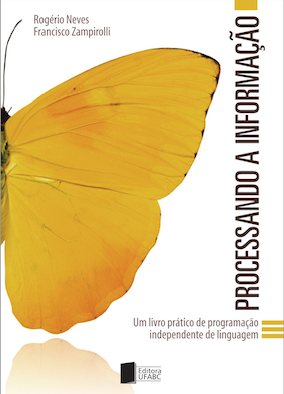
\includegraphics{"figs/Capa_Processando_Informacao.jpg"}

Este caderno (Notebook) é parte complementar \emph{online} do livro
\textbf{\href{https://editora.ufabc.edu.br/matematica-e-ciencias-da-computacao/58-processando-a-informacao}{Processando
a Informação}: um livro prático de programação independente de
linguagem}, que deve ser consultado no caso de dúvidas sobre os temas
apresentados.

\begin{quote}
Este conteúdo pode ser copiado e alterado livremente e foi inspirado
nesse livro.
\end{quote}

    \hypertarget{sumuxe1rio}{%
\subsection{Sumário}\label{sumuxe1rio}}

\begin{itemize}
\tightlist
\item
  Revisão do capítulo anterior
\item
  Introdução
\item
  Instanciando matrizes
\item
  Acessando elementos de uma matriz
\item
  Formas de percorrer uma matriz
\item
  Aplicações usando matrizes
\item
  Revisão deste capítulo
\item
  Exercícios
\end{itemize}

    \hypertarget{revisuxe3o-do-capuxedtulo-anterior-vetores}{%
\subsection{Revisão do capítulo anterior
(Vetores)}\label{revisuxe3o-do-capuxedtulo-anterior-vetores}}

    \begin{itemize}
\item
  Introdução \textgreater{} Vetores são estruturas para armazenar vários
  elementos de um mesmo tipo de dados em uma única variável.
\item
  Trabalhando com vetores \textgreater{} Cada linguagem possui uma
  sintaxe própria para declarar e alocar vetores.
\item
  Acessando elementos de um vetor \textgreater{} \textbf{ATENÇÃO} para
  não acessar uma posição do vetor não reservada/alocada, geralmente
  \texttt{\textless{}0} e \texttt{\textgreater{}=n}.
\item
  Formas de percorrer um vetor \textgreater{} É possível varrer um vetor
  na forma \textbf{\emph{raster}} e \textbf{\emph{anti-raster}}, também
  usando diferentes passos, mas geralmente é passo=1.
\item
  Modularização e vetores \textgreater{} Muito útil usar principalmente
  os módulos de \texttt{leiaVetor} e \texttt{escrevaVetor}, podendo ser
  reaproveitados em vários códigos.
\item
  Tudo que foi visto no capítulo anterior de \textbf{Vetores} (ou
  estruturas \textbf{unidimensional} ou \textbf{1D}) se estende a
  estrutura de \textbf{Matrizes} (ou estruturas \textbf{bidimensional}
  ou \textbf{2D)}).
\end{itemize}

    \hypertarget{introduuxe7uxe3o}{%
\subsection{Introdução}\label{introduuxe7uxe3o}}

    \begin{itemize}
\item
  Existem situações onde é necessário estender a definição de vetor para
  mais de uma dimensão de dados.
\item
  Por exemplo, uma forma muito utilizada de manipulação de dados é em
  tabelas.
\item
  Como exemplo, para listar todos os alunos de uma turma e suas notas em
  uma disciplina,

  \begin{itemize}
  \tightlist
  \item
    as linhas da tabela podem armazenar a identificação dos alunos na
    primeira coluna,
  \item
    nas colunas seguintes podem armazenar as notas da prova1, prova2,
    projeto e, numa última coluna, podem armazenar a nota final do
    aluno.
  \end{itemize}
\item
  Analogamente a um vetor, em uma matriz cada elemento possui apenas um
  dado.
\item
  Além disso, na maioria das linguagens de programação, todos os
  elementos de uma matriz são de um mesmo tipo de dado.
\end{itemize}

    \begin{itemize}
\item
  Um outro exemplo de matrizes muito usado, especialmente com a
  popularização dos dispositivos móveis como celulares e \emph{tablets},
  que comumente trazem câmeras digitais acopladas, ocorre no
  armazenamento e processamento digital de imagens.
\item
  Mas antes das câmeras digitais, já havia \emph{scanners} e
  digitalizadores, e uma imagem pode ser representada por uma
  \textbf{matriz} em um computador.
\item
  Veja o conteúdo no \textbf{\emph{QRCode}} (imagem=matriz) abaixo
  usando um aplicativo leitor de QRCode, disponível para
  \emph{Smartphones} (teste nesta imagem).
\item
  O conteúdo do \textbf{\emph{QRCode}} direciona para uma página
  \emph{web} mostrando uma imagem colorida.
\item
  As imagens coloridas podem ser armazenada em uma estrutura de matriz
  \textbf{tridimensional}, onde cada dimensão armazena uma matriz para
  uma cor primária (RGB - \emph{Red-Green-Blue} ou vermelhor, verde e
  azul).
\end{itemize}


\includegraphics{"figs/image38.png"}

    \begin{figure}
\centering
\caption{image.png}
\end{figure}

    \hypertarget{instanciando-matrizes}{%
\subsection{Instanciando Matrizes}\label{instanciando-matrizes}}

    \begin{itemize}
\item
  Nas linguagens MatLab e R, uma matriz é definida com elementos da
  posição \texttt{(1,1)} até a posição \texttt{(L,\ C)}, onde \texttt{L}
  representa o número de linhas e \texttt{C} representa o número de
  colunas de uma matriz.
\item
  Na maioria das linhagens de programação, no entanto, o índice começa
  no zero, sendo os elementos de uma matriz armazenados da posição
  \texttt{(0,0)} até \texttt{(L-1,C-1)}.
\item
  Nos exemplos a seguir são apresentados alguns exemplos de instanciação
  de matrizes em diferentes linguagens de programação.
\end{itemize}

    \hypertarget{acessando-elementos-de-uma-matriz}{%
\subsection{Acessando elementos de uma
matriz}\label{acessando-elementos-de-uma-matriz}}

    \begin{itemize}
\tightlist
\item
  Uma matriz está pronta para se inserir elementos ou se alterar seus
  dados após instanciada e alocada na memória, em todas as suas
  dimensões.
\item
  Veja uma forma de visualizar uma matriz 2D na Figura abaixo.
\end{itemize}

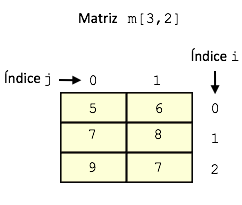
\includegraphics{"figs/image40.png"}

    \begin{figure}
\centering
\caption{image.png}
\end{figure}

    \begin{itemize}
\tightlist
\item
  Essa figura ilustra uma matriz com \texttt{3} linhas e \texttt{2}
  colunas.
\item
  Para visualizar seus elementos podemos usar os índices \texttt{i} e
  \texttt{j},

  \begin{itemize}
  \tightlist
  \item
    com valores para as linhas \texttt{0\textless{}=i\textless{}3} e
  \item
    para as colunas \texttt{0\textless{}=j\textless{}2}.
  \end{itemize}
\item
  Analogamente ao vetor, mas com uma dimensão a mais, a matriz recebe
  valores para os seus elementos, conforme a seguinte estrutura em
  pseudocódigo:
\end{itemize}

    \begin{verbatim}
Instanciar uma matriz m com 3 linhas e 2 colunas
m[0,0] = 5 # linha i=0
m[0,1] = 6
m[1,0] = 7 # linha i=1
m[1,1] = 8
m[2,0] = 9 # linha i=2
m[2,1] = 7
\end{verbatim}

    \hypertarget{formas-de-se-percorrer-uma-matriz}{%
\subsection{Formas de se percorrer uma
matriz}\label{formas-de-se-percorrer-uma-matriz}}

    \begin{itemize}
\tightlist
\item
  Analogamente ao vetor, uma matriz, após criada, possui tamanho fixo.
\item
  Geralmente, para cada dimensão da matriz, é recomendado usar uma
  estrutura de repetição \texttt{para}, \textgreater{} com o objetivo de
  tornar o código mais compacto e genérico para matrizes de quaisquer
  dimensões.
\item
  Além disso, é natural percorrer (ou varrer) a matriz

  \begin{itemize}
  \tightlist
  \item
    da linha \texttt{i=0} até a linha \texttt{i\textless{}L}, onde L
    representa o número de linhas de uma matriz.
  \item
    e da coluna \texttt{j=0} até a coluna \texttt{j\textless{}C}.
  \end{itemize}
\item
  No exemplo a seguir em pseudocódigo, uma matriz \texttt{m} é criada
  com \texttt{6} elementos, sendo três linhas e \texttt{2} colunas, e os
  dois laços \texttt{para} inicializam todos os seus elementos com o
  valor 0.
\end{itemize}

    \begin{verbatim}
Instanciar uma matriz m com 3 linhas e 2 colunas 
inteiros L=3, C=2
Para cada i, de i=0; até i<L; passo i=i+1 faça
    Para cada j, de j=0; até j<C; passo j=j+1 faça
        m[i,j] = 0
\end{verbatim}

    \begin{itemize}
\item
  Existem várias formas de percorrer (ou varrer) uma matriz usando uma
  estrutura de repetição.
\item
  Por exemplo, é possível percorrer uma matriz

  \begin{itemize}
  \tightlist
  \item
    do primeiro elemento \texttt{m{[}0,0{]}} \textgreater{}
    (convencionando como canto superior esquerdo)
  \item
    até o último elemento \texttt{m{[}L-1,C-1{]}} \textgreater{}
    (convencionando como canto inferior direito da matriz),
  \item
    linha por linha, ou coluna por coluna.
  \end{itemize}
\item
  Esse tipo de varredura é chamada \textbf{\emph{raster}}.
\item
  A varredura inversa é chamada \textbf{\emph{anti-raster}}, do último
  elemento inferior direito, até o primeiro elemento superior esquerdo.
\end{itemize}

    \hypertarget{exemplo-01---lerescrever-matriz}{%
\subsection{Exemplo 01 - Ler/Escrever
matriz}\label{exemplo-01---lerescrever-matriz}}

    \begin{itemize}
\item
  Analogamente ao que foi feito no capítulo anterior sobre vetores, onde
  alocamos os vetores em tempo de execução através de métodos, é
  possível usar modularização para melhorar a organização, manutenção e
  reaproveitamento de código.
\item
  Aqui é apresentado um método \texttt{leiaMatriz} e
  \texttt{escrevaMatriz} genéricos
\item
  Para entrada de dados, ou seja, inserir valores nos elementos alocados
  na memória para uma matriz.
\item
  Além de saída de dados, para escrever a matriz, linha por linha.
\end{itemize}

    \hypertarget{pseudocuxf3digo}{%
\paragraph{Pseudocódigo}\label{pseudocuxf3digo}}

    \textbf{Exemplo 01:} Considere um algoritmo para: * Ler um inteiro
\texttt{L} (linhas) representando o número de alunos, * Ler um inteiro
\texttt{C} representando o número de avaliações. * Considere a primeira
coluna o \texttt{RA} do aluno, assim \texttt{C=C+1}. * Criar uma matriz
\texttt{m} com dimensões \texttt{LxC}. * Ler todos os elementos da
matriz. * Escrever todos os elementos da matriz, formando a saída, linha
por linha, por exemplo, para uma matriz com \texttt{2} alunos e
\texttt{3} avaliações, escreva:

\begin{verbatim}
LISTA DE ALUNOS vs Avaliações:
1234 4 3 9
3456 6 4 8
\end{verbatim}

    \begin{verbatim}
Função inteiro m[][] leiaMatriz(inteiro L, inteiro C):
    Instanciar e alocar uma matriz m de Reais com L x C
    Para cada i, de i=0; até i<L; passo i=i+1 faça
        Para cada j, de j=0; até j<C; passo j=j+1 faça
            m[i,j] = leia("Digite um número inteiro:");

Função escrevaMatriz(inteiro m[][], inteiro L, inteiro C): 
    Instanciar e alocar uma matriz m de Reais com L x C
    Para cada i, de i=0; até i<L; passo i=i+1 faça
        Para cada j, de j=0; até j<C; passo j=j+1 faça
            escreva(" ", m[i,j]);
        escreva("\n"); // pula linha

// PROGRAMA PRINCIPAL
// ENTRADAS
inteiro L = leia("Digite o numero de alunos:")
inteiro C = leia("Digite o numero de avaliações:")
C = C + 1  // a primeira coluna é o RA
Instanciar uma matriz m com L linhas e C colunas 

m = leiaMatriz(L,C)
// PROCESSAMENTO: ?

// SAÍDA
escrevaMatriz(m)
\end{verbatim}

    \hypertarget{casos-para-teste-moodlevpl}{%
\paragraph{Casos para Teste
Moodle+VPL}\label{casos-para-teste-moodlevpl}}

Para o professor criar uma atividade VPL no Moodle para este Exemplo 01,
basta incluir em \texttt{Casos\ para\ teste}, o seguinte texto (pode
incluir mais casos):

\begin{verbatim}
case=caso1
input=2
3
1234 
4 
3 
9
3456
6
4
8
output=
LISTA DE ALUNOS vs Avaliações:
1234 4 3 9
3456 6 4 8
\end{verbatim}

    \begin{tcolorbox}[breakable, size=fbox, boxrule=1pt, pad at break*=1mm,colback=cellbackground, colframe=cellborder]
\prompt{In}{incolor}{ }{\boxspacing}
\begin{Verbatim}[commandchars=\\\{\}]
\PY{o}{\PYZpc{}\PYZpc{}writefile} cap6ex01.c
\PY{c+c1}{\PYZsh{}include \PYZlt{}stdio.h\PYZgt{}}
\PY{c+c1}{\PYZsh{}include\PYZlt{}malloc.h\PYZgt{}  }

\PY{n+nb}{int} \PY{o}{*}\PY{o}{*} \PY{n}{leiaMatriz}\PY{p}{(}\PY{n+nb}{int} \PY{n}{L}\PY{p}{,} \PY{n+nb}{int} \PY{n}{C}\PY{p}{)} \PY{p}{\PYZob{}}
  \PY{n+nb}{int} \PY{o}{*}\PY{o}{*}\PY{n}{m} \PY{o}{=} \PY{p}{(}\PY{n+nb}{int} \PY{o}{*}\PY{o}{*}\PY{p}{)}\PY{n}{malloc}\PY{p}{(}\PY{n}{L}\PY{o}{*}\PY{n}{sizeof}\PY{p}{(}\PY{n+nb}{int}\PY{o}{*}\PY{p}{)}\PY{p}{)}\PY{p}{;} 
  \PY{k}{for} \PY{p}{(}\PY{n+nb}{int} \PY{n}{i} \PY{o}{=} \PY{l+m+mi}{0}\PY{p}{;} \PY{n}{i} \PY{o}{\PYZlt{}} \PY{n}{L}\PY{p}{;} \PY{n}{i}\PY{o}{+}\PY{o}{+}\PY{p}{)} \PY{p}{\PYZob{}}
    \PY{n}{m}\PY{p}{[}\PY{n}{i}\PY{p}{]} \PY{o}{=} \PY{p}{(}\PY{n+nb}{int} \PY{o}{*}\PY{p}{)}\PY{n}{malloc}\PY{p}{(}\PY{n}{C} \PY{o}{*} \PY{n}{sizeof}\PY{p}{(}\PY{n+nb}{int}\PY{p}{)}\PY{p}{)}\PY{p}{;} \PY{o}{/}\PY{o}{/} \PY{k}{for} \PY{n}{each} \PY{n}{row} \PY{n}{allocate} \PY{n}{C} \PY{n}{ints}
    \PY{k}{for} \PY{p}{(}\PY{n+nb}{int} \PY{n}{j} \PY{o}{=} \PY{l+m+mi}{0}\PY{p}{;} \PY{n}{j} \PY{o}{\PYZlt{}} \PY{n}{C}\PY{p}{;} \PY{n}{j}\PY{o}{+}\PY{o}{+}\PY{p}{)} 
      \PY{n}{scanf}\PY{p}{(}\PY{l+s+s2}{\PYZdq{}}\PY{l+s+si}{\PYZpc{}d}\PY{l+s+s2}{\PYZdq{}}\PY{p}{,} \PY{o}{\PYZam{}}\PY{n}{m}\PY{p}{[}\PY{n}{i}\PY{p}{]}\PY{p}{[}\PY{n}{j}\PY{p}{]}\PY{p}{)}\PY{p}{;} 
  \PY{p}{\PYZcb{}}
  \PY{k}{return} \PY{n}{m}\PY{p}{;}
\PY{p}{\PYZcb{}}
\PY{n}{void} \PY{n}{free\PYZus{}matrix}\PY{p}{(}\PY{n+nb}{int} \PY{o}{*}\PY{o}{*}\PY{n}{m}\PY{p}{,} \PY{n+nb}{int} \PY{n}{L}\PY{p}{)} \PY{p}{\PYZob{}}
    \PY{k}{for} \PY{p}{(}\PY{n+nb}{int} \PY{n}{i} \PY{o}{=} \PY{l+m+mi}{0}\PY{p}{;} \PY{n}{i} \PY{o}{\PYZlt{}} \PY{n}{L}\PY{p}{;} \PY{n}{i}\PY{o}{+}\PY{o}{+}\PY{p}{)} 
         \PY{n}{free}\PY{p}{(}\PY{n}{m}\PY{p}{[}\PY{n}{i}\PY{p}{]}\PY{p}{)}\PY{p}{;}
    \PY{n}{free}\PY{p}{(}\PY{n}{m}\PY{p}{)}\PY{p}{;}
 \PY{p}{\PYZcb{}}
\PY{n}{void} \PY{n}{escrevaMatriz}\PY{p}{(}\PY{n+nb}{int} \PY{o}{*}\PY{o}{*}\PY{n}{m}\PY{p}{,} \PY{n+nb}{int} \PY{n}{L}\PY{p}{,} \PY{n+nb}{int} \PY{n}{C}\PY{p}{)} \PY{p}{\PYZob{}}
  \PY{k}{for} \PY{p}{(}\PY{n+nb}{int} \PY{n}{i} \PY{o}{=} \PY{l+m+mi}{0}\PY{p}{;} \PY{n}{i} \PY{o}{\PYZlt{}} \PY{n}{L}\PY{p}{;} \PY{n}{i}\PY{o}{+}\PY{o}{+}\PY{p}{)} \PY{p}{\PYZob{}}
   \PY{k}{for} \PY{p}{(}\PY{n+nb}{int} \PY{n}{j} \PY{o}{=} \PY{l+m+mi}{0}\PY{p}{;} \PY{n}{j} \PY{o}{\PYZlt{}} \PY{n}{C}\PY{p}{;} \PY{n}{j}\PY{o}{+}\PY{o}{+}\PY{p}{)} 
      \PY{n}{printf}\PY{p}{(}\PY{l+s+s2}{\PYZdq{}}\PY{l+s+si}{\PYZpc{}d}\PY{l+s+se}{\PYZbs{}t}\PY{l+s+s2}{\PYZdq{}}\PY{p}{,} \PY{n}{m}\PY{p}{[}\PY{n}{i}\PY{p}{]}\PY{p}{[}\PY{n}{j}\PY{p}{]}\PY{p}{)}\PY{p}{;} 
   \PY{n}{printf}\PY{p}{(}\PY{l+s+s2}{\PYZdq{}}\PY{l+s+se}{\PYZbs{}n}\PY{l+s+s2}{\PYZdq{}}\PY{p}{)}\PY{p}{;}
  \PY{p}{\PYZcb{}}
\PY{p}{\PYZcb{}}
\PY{n+nb}{int} \PY{n}{main}\PY{p}{(}\PY{n}{void}\PY{p}{)} \PY{p}{\PYZob{}}
  \PY{o}{/}\PY{o}{/} \PY{n}{ENTRADA} \PY{n}{DE} \PY{n}{DADOS}
  \PY{n+nb}{int} \PY{n}{L}\PY{p}{,} \PY{n}{C}\PY{p}{,} \PY{o}{*}\PY{o}{*}\PY{n}{m}\PY{p}{;}   \PY{o}{/}\PY{o}{/} \PY{n}{variaveis} \PY{n}{de} \PY{n}{referência} \PY{n}{m}
  \PY{n}{printf}\PY{p}{(}\PY{l+s+s2}{\PYZdq{}}\PY{l+s+s2}{Digite o número de alunos: }\PY{l+s+s2}{\PYZdq{}}\PY{p}{)}\PY{p}{;}
  \PY{n}{scanf}\PY{p}{(}\PY{l+s+s2}{\PYZdq{}}\PY{l+s+si}{\PYZpc{}d}\PY{l+s+s2}{\PYZdq{}}\PY{p}{,} \PY{o}{\PYZam{}}\PY{n}{L}\PY{p}{)}\PY{p}{;}

  \PY{n}{printf}\PY{p}{(}\PY{l+s+s2}{\PYZdq{}}\PY{l+s+s2}{Digite o número de avaliações: }\PY{l+s+s2}{\PYZdq{}}\PY{p}{)}\PY{p}{;}
  \PY{n}{scanf}\PY{p}{(}\PY{l+s+s2}{\PYZdq{}}\PY{l+s+si}{\PYZpc{}d}\PY{l+s+s2}{\PYZdq{}}\PY{p}{,} \PY{o}{\PYZam{}}\PY{n}{C}\PY{p}{)}\PY{p}{;}

  \PY{n}{C} \PY{o}{=} \PY{n}{C} \PY{o}{+} \PY{l+m+mi}{1}\PY{p}{;} \PY{o}{/}\PY{o}{/} \PY{n}{a} \PY{n}{primeira} \PY{n}{coluna} \PY{n}{é} \PY{n}{o} \PY{n}{RA} \PY{n}{do} \PY{n}{aluno}

  \PY{n}{printf}\PY{p}{(}\PY{l+s+s2}{\PYZdq{}}\PY{l+s+s2}{Digite os elementos da matriz}\PY{l+s+s2}{\PYZdq{}}\PY{p}{)}\PY{p}{;}
  \PY{n}{m} \PY{o}{=} \PY{n}{leiaMatriz}\PY{p}{(}\PY{n}{L}\PY{p}{,}\PY{n}{C}\PY{p}{)}\PY{p}{;}

  \PY{o}{/}\PY{o}{/} \PY{n}{PROCESSAMENTO} \PY{err}{?}

  \PY{o}{/}\PY{o}{/} \PY{n}{SAÍDA} \PY{n}{DE} \PY{n}{DADOS}
  \PY{n}{printf}\PY{p}{(}\PY{l+s+s2}{\PYZdq{}}\PY{l+s+se}{\PYZbs{}n}\PY{l+s+s2}{LISTA DE ALUNOS vs Avaliações:}\PY{l+s+se}{\PYZbs{}n}\PY{l+s+s2}{\PYZdq{}}\PY{p}{)}\PY{p}{;}
  \PY{n}{printf}\PY{p}{(}\PY{l+s+s2}{\PYZdq{}}\PY{l+s+s2}{RA }\PY{l+s+s2}{\PYZdq{}}\PY{p}{)}\PY{p}{;}
  \PY{k}{for} \PY{p}{(}\PY{n+nb}{int} \PY{n}{i} \PY{o}{=} \PY{l+m+mi}{0}\PY{p}{;} \PY{n}{i} \PY{o}{\PYZlt{}} \PY{n}{C}\PY{o}{\PYZhy{}}\PY{l+m+mi}{1}\PY{p}{;} \PY{n}{i}\PY{o}{+}\PY{o}{+}\PY{p}{)} 
    \PY{n}{printf}\PY{p}{(}\PY{l+s+s2}{\PYZdq{}}\PY{l+s+se}{\PYZbs{}t}\PY{l+s+si}{\PYZpc{}d}\PY{l+s+s2}{\PYZdq{}}\PY{p}{,}\PY{p}{(}\PY{n}{i}\PY{o}{+}\PY{l+m+mi}{1}\PY{p}{)}\PY{p}{)}\PY{p}{;} 
  
  \PY{n}{printf}\PY{p}{(}\PY{l+s+s2}{\PYZdq{}}\PY{l+s+se}{\PYZbs{}n}\PY{l+s+s2}{\PYZdq{}}\PY{p}{)}\PY{p}{;}
  \PY{n}{escrevaMatriz}\PY{p}{(}\PY{n}{m}\PY{p}{,}\PY{n}{L}\PY{p}{,}\PY{n}{C}\PY{p}{)}\PY{p}{;}
  \PY{n}{free\PYZus{}matrix}\PY{p}{(}\PY{n}{m}\PY{p}{,}\PY{n}{L}\PY{p}{)}\PY{p}{;} \PY{o}{/}\PY{o}{/} \PY{n}{liberar} \PY{n}{memória} \PY{n}{alocado} \PY{n}{com} \PY{n}{malloc}
  \PY{k}{return} \PY{l+m+mi}{0}\PY{p}{;}
\PY{p}{\PYZcb{}}
\end{Verbatim}
\end{tcolorbox}

    \begin{tcolorbox}[breakable, size=fbox, boxrule=1pt, pad at break*=1mm,colback=cellbackground, colframe=cellborder]
\prompt{In}{incolor}{ }{\boxspacing}
\begin{Verbatim}[commandchars=\\\{\}]
\PY{o}{\PYZpc{}\PYZpc{}}\PY{k}{shell}
gcc \PYZhy{}Wall \PYZhy{}std=c99 cap6ex01.c \PYZhy{}o output2
./output2
\end{Verbatim}
\end{tcolorbox}

    \hypertarget{acessando-elemento-com}{%
\subparagraph{\texorpdfstring{Acessando elemento com
\texttt{*}}{Acessando elemento com *}}\label{acessando-elemento-com}}

Outras forma de acessar elementos em matriz.

\begin{verbatim}
  for (int i = 0; i < L; i++) 
   for (int j = 0; j < C; j++) {
      printf("%d\t", m[i][j]); // ou
      printf("%d\t", *(m + i*C + j));
   }
\end{verbatim}

Ou utilizando apenas um laço para varrar uma matriz:

\begin{verbatim}
  for (int i = 0; i < L*C; i++) {
      printf("%d\t", m[i/C][i%C]); // ou
      printf("%d\t", *(m + i));
   }
\end{verbatim}

    \hypertarget{matriz-multimensional}{%
\subparagraph{Matriz Multimensional}\label{matriz-multimensional}}

\begin{verbatim}
for (int k = 0; k < D; k++) // profundidade
  for (int i = 0; i < L; i++) // linha
   for (int j = 0; j < C; j++) { // coluna
      printf("%d\t", m[k][i][j]); // ou
      printf("%d\t", *(m + k*L*C + i*C + j));
   }
\end{verbatim}

Ou utilizando apenas um laço para varrar uma matriz:

\begin{verbatim}
  for (int i = 0; i < D*L*C; i++) {
      d = i/(L*C);
      printf("%d\t", m[d][(d-i)/C][(d-i)%C]); // ou
      printf("%d\t", *(m + i));
   }
\end{verbatim}

    \hypertarget{exercuxedcios}{%
\subsection{Exercícios}\label{exercuxedcios}}

    Ver notebook Colab nos arquivos \texttt{cap6.partX.lab.*.ipynb}
(\texttt{X} \(\in\) \texttt{{[}2,3,4,5{]}} e \texttt{*} é a extensão da
linguagem), utilizando alguma linguagem de programação de sua
preferência, onganizadas em subpastas contidas em \texttt{"gen"}, na
pasta do Google Drive
\href{https://drive.google.com/drive/folders/1YlFwv8XYN7PYYf-HwDMlkxzbmXzJw9cM?usp=sharing}{colabs}.

    \hypertarget{atividades-no-moodlevpl}{%
\subsection{Atividades no Moodle+VPL}\label{atividades-no-moodlevpl}}

Algumas atividades no Moodle+VPL pedem como entradas matrizes de
inteiros (ou reais), \textbf{armazenados em várias linhas}. Exemplo de
entrada a ser lida:

\hypertarget{entrada-de-dados-cada-linha-contem-um-texto-ou-string-com-elementos-da-linha-da-matriz-e-vuxe1rios-espauxe7os}{%
\subsubsection{\texorpdfstring{Entrada de Dados (cada linha contem um
texto ou \emph{string} com elementos da linha da matriz e vários espaços
``\texttt{}''):}{Entrada de Dados (cada linha contem um texto ou string com elementos da linha da matriz e vários espaços ``\,''):}}\label{entrada-de-dados-cada-linha-contem-um-texto-ou-string-com-elementos-da-linha-da-matriz-e-vuxe1rios-espauxe7os}}

\begin{verbatim}
0 9 3 6 9 8 4 5 4
8 1 2 3 5 2 9 9 6
4 1 1 0 9 9 8 2 7
5 2 8 4 6 6 0 8 0
4 7 6 4 3 9 3 3 5
2 6 0 4 0 7 5 5 2
9 8 4 8 4 7 1 4 3
\end{verbatim}

Para não ter que incluir várias entradas inteiras, a melhor solução é
fazer um método de leitura, passando como argumento um texto
(\emph{string}) com várias linhas. O final de cada linha é definido por
\texttt{\textbackslash{}n} e o final da matriz deve ser uma linha em
branco com apenas \texttt{\textbackslash{}n}. Esse método deve retornar
a matriz.

    \hypertarget{revisuxe3o-deste-capuxedtulo-de-matriz}{%
\subsection{Revisão deste capítulo de
Matriz}\label{revisuxe3o-deste-capuxedtulo-de-matriz}}

\begin{itemize}
\tightlist
\item
  Introdução
\item
  Instanciando matrizes
\item
  Acessando elementos de uma matriz
\item
  Formas de percorrer uma matriz
\item
  Aplicações usando matrizes
\item
  Exercícios
\item
  Revisão deste capítulo de Matriz
\end{itemize}


    % Add a bibliography block to the postdoc
    
    
    
\end{document}
